
反向迭代器适配器是反转迭代器类方向的抽象,需要是一个双向迭代器。

\subsubsection{How to do it…}

STL中的大多数双向容器都包含一个反向迭代器适配器。其他容器则没有,如原始C数组。来看一些例子:

\begin{itemize}
\item 
从本章一直使用的printc()函数开始:

\begin{lstlisting}[style=styleCXX]
void printc(const auto & c, const string_view s = "") {
	if(s.size()) cout << format("{}: ", s);
	for(auto e : c) cout << format("{} ", e);
	cout << '\n';
}
\end{lstlisting}

使用一个基于范围的for循环来打印容器的元素。

\item 
基于范围的for循环,甚至适用于没有迭代器类的C数组。因此,printc()函数也适用于C数组:

\begin{lstlisting}[style=styleCXX]
int main() {
	int array[]{ 1, 2, 3, 4, 5 };
	printc(array, "c-array");
}
\end{lstlisting}

会得到这样的输出:

\begin{tcblisting}{commandshell={}}
c-array: 1 2 3 4 5
\end{tcblisting}

\item 
可以使用begin()和end()迭代器适配器为C数组创建普通的前向迭代器:

\begin{lstlisting}[style=styleCXX]
auto it = std::begin(array);
auto end_it = std::end(array);
while (it != end_it) {
	cout << format("{} ", *it++);
}
\end{lstlisting}

for循环的输出为:

\begin{tcblisting}{commandshell={}}
1 2 3 4 5
\end{tcblisting}

\item 
或者使用rbegin()和rend()反向迭代器适配器为C数组创建反向迭代器:

\begin{lstlisting}[style=styleCXX]
auto it = std::rbegin(array);
auto end_it = std::rend(array);
while (it != end_it) {
	cout << format("{} ", *it++);
}
\end{lstlisting}

现在输出反过来了:

\begin{tcblisting}{commandshell={}}
5 4 3 2 1
\end{tcblisting}

\item 
甚至可以创建另一个printr(),进行反向打印:

\begin{lstlisting}[style=styleCXX]
void printr(const auto & c, const string_view s = "") {
	if(s.size()) cout << format("{}: ", s);
	auto rbegin = std::rbegin(c);
	auto rend = std::rend(c);
	for(auto it = rbegin; it != rend; ++it) {
		cout << format("{} ", *it);
	}
	cout << '\n';
}
\end{lstlisting}

当用C数组使用时:

\begin{lstlisting}[style=styleCXX]
printr(array, "rev c-array");
\end{lstlisting}

会得到这样的输出:

\begin{tcblisting}{commandshell={}}
rev c-array: 5 4 3 2 1
\end{tcblisting}

\item 
当然,这也适用于双向STL容器:

\begin{lstlisting}[style=styleCXX]
vector<int> v{ 1, 2, 3, 4, 5 };
printc(v, "vector");
printr(v, "rev vector");
\end{lstlisting}

输出为:

\begin{tcblisting}{commandshell={}}
vector: 1 2 3 4 5
rev vector: 5 4 3 2 1
\end{tcblisting}
\end{itemize}


\subsubsection{How it works…}

普通的迭代器类有一个begin()迭代器指向第一个元素,还有一个end()迭代器指向最后一个元素之后:

\hspace*{\fill} \\ %插入空行
\begin{center}
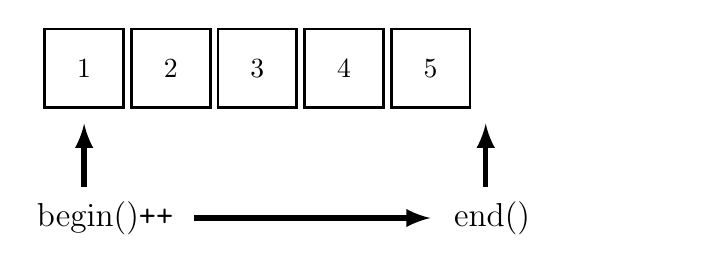
\begin{tikzpicture}
\foreach \x in {1,...,5} {
	\draw[line width=1pt] (1.1*\x,1) rectangle (1.1*\x+1,0) node[pos=.5] {\x};
}

\draw[line width=2pt][-latex] (1.6,-1.0) -- (1.6,-0.2);
\draw[line width=2pt][-latex] (6.7,-1.0) -- (6.7,-0.2);

\node[text width=3cm, font=\large] at (2.5,-1.4) {begin()\texttt{++}};
\node[text width=3cm, font=\large] at (7.8,-1.4) {end()};

\draw[line width=2pt][-latex] (3,-1.4) -- (6.0,-1.4);
\end{tikzpicture}

图4.3 前向迭代器
\end{center}

通过使用自加操作符递增begin()迭代器来迭代容器,直到end()迭代器的值。

反向迭代器适配器拦截迭代器接口,并将其反转。使begin()迭代器指向最后一个元素,end()迭代器指向第一个元素之前。++和--操作符也是颠倒的:

\hspace*{\fill} \\ %插入空行
\begin{center}
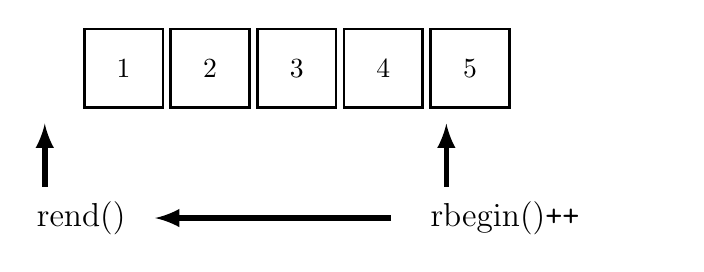
\begin{tikzpicture}
\foreach \x in {1,...,5} {
	\draw[line width=1pt] (1.1*\x,1) rectangle (1.1*\x+1,0) node[pos=.5] {\x};
}

\draw[line width=2pt][-latex] (0.6,-1.0) -- (0.6,-0.2);
\draw[line width=2pt][-latex] (5.7,-1.0) -- (5.7,-0.2);

\node[text width=3cm, font=\large] at (2.0,-1.4) {rend()};
\node[text width=3cm, font=\large] at (7.0,-1.4) {rbegin()\texttt{++}};

\draw[line width=2pt][-latex] (5.0,-1.4) -- (2,-1.4);
\end{tikzpicture}

图4.4 反向迭代器适配器
\end{center}


反向迭代器中,++操作符递减,-{}-操作符递增。

大多数双向STL容器已经包含了一个反向迭代器适配器,可以通过成员函数rbegin()和rend()访问:

\begin{lstlisting}[style=styleCXX]
vector<int> v;
it = v.rbegin();
it_end = v.rend();
\end{lstlisting}

这些迭代器将反向操作,可以用于多种场景。
